\chapter{Параметрическое программирование}\label{chap2}

Сообщество исследователей операций рассматривает вариации параметров в математических программах на двух уровнях: анализ чувствительности, который характеризует изменение решения относительно малых возмущений параметров, и параметрическое программирование, где характеристика решения ищется для полного диапазона значений параметров. Программы, которые зависят только от одного скалярного параметра, называются параметрическими программами, а задачи, зависящие от вектора параметров, называются многопараметрическими программами.

Есть несколько причин для поиска эффективных решений многопараметрических программ. Как правило, математические программы подвержены неопределенности из-за факторов, которые либо неизвестны, либо будут решены позже. Параметрическое программирование систематически подразделяет пространство параметров на характерные области, которые изображают выполнимость и соответствующие характеристики в зависимости от неопределенных параметров, и, следовательно, предоставляют лицу, принимающему решение, полную карту различных результатов.

Наш интерес к многопараметрическому программированию проистекает из области теории систем и оптимального управления. Для динамических систем с дискретным временем задачи оптимального управления с конечными временными ограничениями могут быть сформулированы как математические программы, в которых функция затрат и ограничения являются функциями начального состояния динамической системы. В частности, Заде и Уэйлен, по-видимому, были первыми, кто выразил задачу оптимального управления для линейных систем с ограниченным дискретным временем в виде линейной программы. Используя мультипараметрическое программирование, мы можем охарактеризовать и вычислить решение задачи оптимального управления в явном виде в зависимости от начального состояния.

Нас также мотивирует так называемая методика прогнозного управления моделью (MPC). MPC очень популярен в перерабатывающей промышленности для автоматического регулирования технологических агрегатов в условиях эксплуатации и привлекает значительные исследовательские усилия в последнее десятилетие. MPC требует, чтобы задача оптимизации была решена в режиме онлайн для вычисления следующего командного действия. Такая проблема оптимизации зависит от текущих измерений датчика. Усилия по вычислению могут быть перемещены в автономный режим путем решения многопараметрических программ, где входные данные команды являются переменными оптимизации, а измерения - параметрами.


%%%%%%%%%%%%%%%%%%%%%%%%%%%%%%%%%%%%%%%%%%%%%%%%%%%%%%%%%%%%%%%%%%%%%%%%%%%%%%%%
\section{Многопараметрическое программирование}\label{2sec:gabella}
%%%%%%%%%%%%%%%%%%%%%%%%%%%%%%%%%%%%%%%%%%%%%%%%%%%%%%%%%%%%%%%%%%%%%%%%%%%%%%%%

Вариации параметров в математических программах рассматриваются на двух уровнях: анализ чувствительности, который характеризует изменение решения относительно малых возмущений параметров, и параметрическое программирование, где ищется характеристика решения для полного диапазона значений параметров. Точнее, программы, которые зависят только от одного скалярного параметра, называются параметрическими программами, а задачи, зависящие от вектора параметров, называются многопараметрическими программами.

Интерес к многопараметрическому программированию берет свое начало из области теории систем и оптимального управления. Для динамических систем с дискретным временем конечные задачи оптимального управления с ограничением по времени могут быть сформулированы в виде математических программ, в которых функция стоимости и ограничения являются функциями начального состояния динамической системы.

Используя многопараметрическое программирование, мы можем охарактеризовать и вычислить решение задачи оптимального управления в явном виде как функцию начального состояния.

Нас также мотивирует так называемая методика прогнозного управления моделью (MPC). MPC очень популярен в обрабатывающей промышленности для автоматического регулирования технологических агрегатов в условиях эксплуатации.

MPC требует, чтобы проблема оптимизации была решена в реальном времени для вычисления следующего управляющего воздействия. Такая проблема оптимизации зависит от текущих измерений датчика. Вычислительная точка может быть перемещена в линию путем решения многопараметрических программ, где входные данные команды являются переменными оптимизации, а измерения - параметрами.

Первый метод решения параметрических линейных программ был предложен Гассом и Саати.


Многопараметрический анализ использует концепцию критической области. При заданной параметрической программе критической областью является набор параметров пространства, где локальные условия оптимальности остаются неизменными.

Первый метод решения многопараметрических линейных программ был сформулирован Галом и Недомой.

Первый метод решения многопараметрических квадратичных программ был предложен Бемпорадом.

В этой главе мы сначала напомним основные результаты нелинейного многопараметрического программирования, затем опишем три алгоритма решения многопараметрических линейных программ (mp-LP), многопараметрических квадратичных программ (mp-QP).

Основная идея трех многопараметрических алгоритмов, представленных в этой главе, состоит в том, чтобы построить критическую область в окрестности заданного параметра, используя необходимые и достаточные условия оптимальности, а затем рекурсивно исследовать пространство параметров вне такой области.

Все алгоритмы чрезвычайно просты в реализации, если доступны стандартные солверы задач нелинейного программирования.


%%%%%%%%%%%%%%%%%%%%%%%%%%%%%%%%%%%%%%%%%%%%%%%%%%%%%%%%%%%%%%%%%%%%%%%%%%%%%%%%
\section{Общие результаты для многопараметрических нелинейных программ}\label{2sec:results-multy-parametric}
%%%%%%%%%%%%%%%%%%%%%%%%%%%%%%%%%%%%%%%%%%%%%%%%%%%%%%%%%%%%%%%%%%%%%%%%%%%%%%%%

Рассмотрим нелинейную математическую программу, зависящую от параметра $x$, появляющегося в функции стоимости и в ограничениях

\begin{equation} \label{1function}
   J^*(u) = \inf_{z}f(z,x)
\end{equation}

где $z \in M \subseteq \mathbb{R}^s$ --- переменная оптимизации,\ $x \in X \subseteq R^n$ --- параметр,\ $f: \mathbb{R}^s\times\mathbb{R}^n \to \mathbb{R}$ --- функция стоимости, а $g: \mathbb{R}^s\times\mathbb{R}^n \to R^{n_g}$ --- ограничения.

Небольшое возмущение параметра $x$ в задаче математического программирования (\ref{1function}) может привести к различным результатам. В зависимости от свойств функций $f$ и $g$ решение $z^*(x)$ может плавно или резко меняться в зависимости от $x$. Обозначим через $R(x)$ отображение, которое присваивает параметру $x$ множество выполнимых $z$, т.е.
\begin{equation} \label{2function}
    R(x) = \{z \in M \ |\  g(z,x) < 0 \}.
\end{equation}

$K^*$ --- множество возможных параметров, т. е.
\begin{equation} \label{3function}
    K^* = \{x \in \mathbb{R}^n \ |\  R(x) \not= \varnothing \}.
\end{equation}

$J^*(x)$ --- функция, которая выражает зависимость от $x$ минимального значения целевой функции над $K^*$, т.е.
\begin{equation} \label{4function}
    J^*(x) = \inf_{z}\{f(z,x) \ | \ z \in R(x) \}
\end{equation}

$Z^*(x)$ --- отображение точки-множества, которое выражает зависимость от $x$ множества оптимизаторов, т.е.
\begin{equation} \label{5function}
    Z^*(x) = \{ z \in R(x) \ | \ f(z,x) \leq J^*(x) \}
\end{equation}


$J^*(x)$ будет упоминаться как функция оптимального значения или просто функция значения, $Z^*(x)$ будет упоминаться как оптимальное множество. Если $Z^*(x)$ является синглетоном для всех $x$, то $z^*(x) \triangleq Z^*(x)$ будет называться функцией оптимизатора. Будем предполагать, что $K^*$ замкнуто и $J^*(x)$ конечно для каждого $x$, принадлежащего $K^*$. Обозначим через $g_{i}(z, x)$ $i$-ую компоненту вектор-функции $g(x, z)$.

%определение
\begin{definition}
    $R(x)$ открыто в точке $\overline{x} \in K^*$, если $\{ x^{k} \subset K^*,\ x^{k} \to \overline{x} \}$ и $\overline{z} \in R(\overline{x})$
    подразумевают существование целого числа $m$ и последовательности $\{ z^{k} \in M \}$ такой, что $z^{k} \in R(x^{k})$ при $k \geq m$ и $z^{k} \to \overline{z}$
\end{definition}


\begin{definition}
    $R(x)$ замкнуто в точке $\overline{x} \in K^*$, если $\{ x^{k}\subset K^*,\ x^{k} \to \overline{x},\ z^{k} \in R(x^{k}) \}$, и $z^{k} \to \overline{z}$ влечет  $\overline{z} \in R(\overline{x})$
\end{definition}


\begin{definition}
    $R(x)$ непрерывна в точке $\overline{x} \in K^*$, если она открыта и замкнута в точке $\overline{x}$. $R$ непрерывна в $K^*$, если $R$ непрерывна для любого $x$ из $K^*$.
\end{definition}

%теорема
\begin{theorem}\label{1theorem}
    Если $M$ выпуклая, если каждая компонента $g_{i} (z, x)$ из $g (z, x)$ непрерывна на $M \times X$ и выпукла по $z$ для каждого фиксированного $x \in X$, и если существует такое $\overline{z}$, что $g(\overline{z}, \overline{x}) < 0$, то $R (x)$ --- непрерывное отображение.
\end{theorem}

%литература%
Доказательство дано в \cite{Hogan}.  Отметим, что выпуклости по $z$ для каждого $x$ недостаточно, чтобы показать непрерывность $R (x)$ всюду в $K^*$.

\begin{theorem}\label{2theorem}
    Если $M$ выпуклая, если каждая компонента $g_{i} (z, x)$ из $g (x, z)$ непрерывна на $M \times X$ и выпукла по $z$ и $x$, то $R (x)$ является непрерывным отображением.
\end{theorem}

Доказательство простое и здесь опущено.\\

Теперь мы готовы дать две основные теоремы о непрерывности функции значения и функции оптимизатора.

\begin{theorem}\label{3theorem}
    Рассмотрим задачу (\ref{1function}) - (\ref{2function}). Если $R (x)$ --- непрерывное отображение точечных множеств и $f (z, x)$ непрерывное, то $J^*(x)$ непрерывно.
\end{theorem}


\begin{theorem}\label{4theorem}
    Рассмотрим задачу (\ref{1function}) - (\ref{2function}). Если $R (x)$ --- непрерывное отображение точечных множеств, $R (x)$ является выпуклым для каждого $x \in K^*,\ f (z, x)$ непрерывныx и строго квазивыпуклыx в $z$ для каждого $x$, то $J^* (x)$ и $z^* (x)$ --- непрерывные функции.
\end{theorem}

Теоремы (\ref{1theorem}) и (\ref{2theorem}) можно объединить с теоремами (\ref{3theorem}) и (\ref{4theorem}), чтобы получить следующие следствия:

%следствие
\begin{corollary}
    Рассмотрим многопараметрическую нелинейную программу (\ref{1function}). Предположим, что $M$ --- компактное выпуклое множество в $R^{s}$,\ $f$ и $g$ непрерывны на $M \times \mathbb{R}^{n}$, и каждая компонента $g$ выпукла на $M \times K^*$. Тогда $J^* (\cdot)$ непрерывно для всех $x \in K^*$.
\end{corollary}

\begin{corollary}
    Рассмотрим многопараметрическую нелинейную программу (\ref{1function}). Предположим, что $M$ --- компактное выпуклое множество в $R^{s}$, $f$ и $g$ непрерывны на $M \times \mathbb{R}^{n}$, и каждая компонента $g$ выпукла на $M$ для каждого $x \in K^*$. Тогда $J^* (x)$ непрерывна в точке $x$, если она существует $\overline{z}$ такая, что $g (\overline{z}, x) < 0$.
\end{corollary}


%%%%%%%%%%%%%%%%%%%%%%%%%%%%%%%%%%%%%%%%%%%%%%%%%%%%%%%%%%%%%%%%%%%%%%%%%%%%%%%%
\section{Многопараметрическое линейное программирование}\label{2sec:darova}
%%%%%%%%%%%%%%%%%%%%%%%%%%%%%%%%%%%%%%%%%%%%%%%%%%%%%%%%%%%%%%%%%%%%%%%%%%%%%%%%

Рассмотрим многопараметрическую линейную программу справа (mp-LP)

\begin{equation}\label{1multy}
    \begin{split}
        J^*(x) = \min_z J(z,x) = c^{'z},\\
        \text{при}\ Gz \leq W + Sx,
    \end{split}
\end{equation}
где $z \in \mathbb{R}^s$ --- переменные оптимизации, $x \in \mathbb{R}^{n}$ --- вектор параметров, $J(z, x) \in \mathbb{R}$ --- целевая функция и $G \in \mathbb{R}^{m \times s},\ c \in \mathbb{R}^{s},\ W \in \mathbb{R}^{m}$, и $S \in \mathbb{R}^{m \times n}$. Для заданного многогранного множества параметров $K \subset R^{n}$,

\begin{equation}\label{2multy}
    K \triangleq \{ x \in \mathbb{R}^{n} : Tx \leq Z \}
\end{equation}

Обозначим через $K^* \subseteq K$ область параметров $x \in K$ такую, что LP (\ref{1multy}) выполнима. Для любого заданного $\overline{x} \in K^*,\ J^*(\cdot)$ обозначает минимальное значение целевой функции в задаче (\ref{1multy}) при $x = \overline{x}$. Функция $J^*: K^* \to \mathbb{R}$ будет обозначать функцию, выражающую зависимость от $x$ минимального значения целевой функции над $K^*$, $J^*(\cdot)$ будем называть функцией значения.
Функция $Z^*: K^* \to 2^{\mathbb{R}^{n}}$, где $2^{\mathbb{R}^{n}}$ --- множество подмножеств $R^{s}$, опишет для любого фиксированного $x \in K^*$ множество оптимизаторов $z^* (x)$, связанных с $J^*(\theta)$. 
Мы стремимся определить допустимую область параметров$K^* \subseteq K$, выражение функции значения и выражение одного из оптимизаторов $z^* (x) \in Z^* (x)$.

Мы даем следующее определение прямой и двойственной невырожденности:

\begin{definition}
    Для любого заданного $x \in K^*$ ЛП (\ref{1multy}) называется прямой невырожденностью, если существует $a\ z^* (x) \in Z^* (x)$ такое, что число активных ограничений в оптимизаторе больше, чем число переменных $s$.
\end{definition}

\begin{definition}
    Для любого данного $x \in K^*$ ЛП (\ref{1multy}) называется двойственной невырожденностью, если его двойственная задача прямая невырожденность.
\end{definition}

Многопараметрический анализ выдвигает концепцию критической области (CR). 
В \cite{Nedoma} критическая область определяется как подмножество пространства параметров, на котором определенный базис линейной программы является оптимальным. 
Алгоритм, предложенный в \cite{Nedoma} для решения многопараметрических линейных программ, генерирует непересекающиеся критические области путем генерации и исследования графа базисов. На графике базисов узлы представляют собой оптимальные базисы данной многопараметрической задачи, и два узла соединены ребром, если можно перейти от одного базиса к другому за один шаг (в этом случае базисы называются соседними). Наше определение критических областей связано не с базисами, а с набором активных ограничений. Ниже мы даем определение оптимального разбиения, непосредственно связанного с делением Филиппи \cite{Filippi}.

Пусть $J \triangleq \{1,..., m\}$ будет набором индексов ограничений. Для любого $A \subseteq J$ пусть $G_{A}$ и $S_A$ - подматрицы $G$ и $S$ соответственно, состоящие из строк, проиндексированных по A, и обозначим через $G_{j},\ S_{j}$ и $W_{j}$ $j$-ую строку $G$, $S$ и $W$, соответственно.


\begin{definition}
    Оптимальным разбиением $J$, связанным с $x$, является разбиение $(A(x), N A(x))$, где

    $$A(x) \triangleq \{ j \in J: G_{j}z^*(x) - S_{j}x = W_{j} \text{для всех} z^*(x) \in Z*(x) \}$$
    $$N A(x) \triangleq \{ j \in J: G_{j}z^*(x) - S_{j}x < W_{j} \text{для некоторых} z^*(x) \in Z*(x) \}$$
\end{definition}
Ясно, что $(A (x), N A(x))$ не пересекаются и их объединением является $J$. Для заданного $x^* \in K^*$ пусть $(A, NA) \triangleq (A (x^*), N A(x^*) )$, и пусть

\begin{equation}\label{3multy}
    \begin{split}
        CR_{A} \triangleq \{ x \in K: A(x) = A \}\\
        \overline{CR_{A}} \triangleq \{ x \in K: A(x) \supseteq A \}.
    \end{split}
\end{equation}
Множество $CR_{A}$ является критической областью, связанной с множеством активных ограничений $A$, то есть множеством всех параметров $x$, таких что ограничения, индексированные по $A$, активны в оптимуме задачи (\ref{1multy}). Ясно, что $\overline{CR_{A}} \supseteq CR_{A}$.


\begin{theorem}\label{5theorem}
    Пусть $(A, NA) \triangleq (A (x^*), NA (x^*))$ для некоторого $x^* \in K$, и пусть $d$ --- размерность области $G_{A}\bigcap S_{A}$. Если $d = 0$, то $CR_{A} = \{x^*\}$. Если $d > 0$, то
    \begin{itemize}
        \item $CR_{A}$ --- открытый многогранник 1 размерности $d^2$;
        \item $\overline{CR_{A}}$ --- замыкание $CR_{A}$;
        \item каждая грань $CR_{A}$ принимает форму $CR_{A}$ для некоторого $A^{'} \supseteq A$.
    \end{itemize}
\end{theorem}

Из теоремы (\ref{5theorem}) и определения критических областей в (\ref{3multy}) следует, что множество $k^*$ всегда разбивается единственным образом. Обратная ситуация в случае вырожденности, в подходе \cite{Gal68} разбиение не определяется однозначно, так как оно может быть сгенерировано экспоненциальным числом способов, в зависимости от конкретного пути, по которому следует алгоритм для посещения различных базисов  \cite{Adler2,Berkelaar28}.

В этой главе мы стремимся определить все полноразмерные критические области, содержащиеся в $K^*$, в соответствии с определением (\ref{3multy}).

Прежде чем идти дальше, вспомним некоторые свойства функции качества $J^* (x): \mathbb{R}^{n} \to \mathbb{R}$ и множества $K^*$.


\begin{theorem}\label{6theorem}
    Предположим, что для фиксированного $x^0 \in K$ существует конечное оптимальное решение $z^* (x_0)$ (\ref{1multy}). Тогда для всех $x \in K$ (\ref{1multy}) имеет либо конечный оптимум, либо выполнимое решение.
\end{theorem}

\begin{theorem}\label{7theorem}
    Пусть $K^* \subseteq K$ --- множество всех параметров $x$, таких что ЛП (\ref{1multy}) имеет конечное оптимальное решение $z^* (x)$. Тогда $K^*$ --- замкнутое полиэдральное множество в $\mathbb{R}^{n}$.
\end{theorem}  

Следующая теорема (\ref{8theorem}) суммирует свойства, которыми обладает многопараметрическое решение \cite{Gal68}.
\begin{theorem}\label{8theorem}
    Функция $J^*(\cdot)$ является выпуклой и кусочно аффинной над $K^*$ (и, в частности, аффинной в каждой критической области $CR_{A_i}$).
    
    Если оптимизатор $z^* (x)$ уникален для всех $x \in K^*$, то функция оптимизатора $z^*: K^* \to R^{s}$ непрерывна и кусочно аффинная. В противном случае всегда можно определить непрерывную и кусочно-аффинную оптимизирующую функцию $z^* (x) \in Z^* (x)$ для всех $z \in K^*$.
\end{theorem}  


В следующей главе мы опишем алгоритм для определения множества $K^*$, его разбиения на полноразмерные критические области $CR_{A_i}$, функцию значения PWA $J^*(\cdot)$ и функции оптимизатора PWA $z^* (\cdot)$.\\

Алгоритм состоит из двух основных этапов, которые можно обобщить следующим образом:
\begin{itemize}
    \item Определите размерность $n^{'} \leq n$ наименьшего аффинного подпространства $\mathcal{K}$, содержащего $K^*$. Если $n^{'} < n$, найдите уравнения в x, которые определяют $\mathcal{K}$.
    \item Определить разбиение $K^*$ на критические области $CR_{A_i}$ и найти функцию $J^* (\cdot)$ и функцию оптимизатора PWA $z^* (\cdot)$.
\end{itemize}

Ниже подробно описывается 2 шага. Первый шаг - предварительный, цель которого состоит в том, чтобы уменьшить количество параметров, чтобы получить полномерную допустимую область параметров. Это облегчает второй шаг, который вычисляет многопараметрическое решение и представляет ядро алгоритма mp-LP.\\

%%%%%%%%%%%%%%%%%%%%%%%%%%%%%%%%%%%%%%%%%%%%%%%%%%%%%%%%%%%%%%%%%%%%%%%%%%%%%%%%
\subsection{Определение аффинного подпространства $\mathcal{K}$}
%%%%%%%%%%%%%%%%%%%%%%%%%%%%%%%%%%%%%%%%%%%%%%%%%%%%%%%%%%%%%%%%%%%%%%%%%%%%%%%%

Чтобы работать с минимальной размерностью вектора параметров, первый шаг алгоритма нацелен на поиск единственного подпространства $\mathcal{K} \subseteq \mathbb{R}^{n}$, содержащего параметры $x$, которые делают (\ref{1multy}) выполнимым.

Первое простое, но важное соображение касается ранга столбца $r_{S}$ в $S$. Понятно, что если параметры $r_{S} < n,\  n - r_{S}$, то можно решить простым преобразованием координат в $\mathbb{R}^{n}$. Поэтому отныне, не теряя общности, будем считать, что $S$ имеет ранг столбца.

Прежде чем решить mp-LP, нам нужен тест для проверки размерности $n$ наименьшего аффинного подпространства $\mathcal{K}$, содержащего $K^*$. Более того, когда $n^{'} < n$, нам нужны уравнения, описывающие $\mathcal{K}$ в $\mathbb{R}^n$. Затем уравнения используются для изменения координат, чтобы уменьшить число параметров с $n$ до $n^{'}$ и получить многогранник $K^*$, который имеет полную размерность в $\mathbb{R}^{n^{'}}$.

Напомним (\ref{1multy}) и построим задачу ЛП в пространстве $\mathbb{R}^{s + n}$

\begin{equation}\label{11multy}
    \begin{split}
        \min_z J(z,x) = c^{'z},\\
        \text{при}\ Gz - Sx \leq W,
    \end{split}
\end{equation}
Ясно, что ограничения в (\ref{11multy}) определяют многогранник $\mathcal{P}$ в $\mathbb{R}^{s + n}$. Следующая лемма показывает, что проекция ${\Pi_{\mathbb{R}^{n}}}(\mathcal{P})$ для $\mathcal{P}$ на пространство параметров $\mathbb{R}^{n}$ есть $K^*$.

\begin{lemma}\label{lemma}
    $x^* \in K^* \Longleftrightarrow \exists z : Gz - Sx^{*} \leq W \Longleftrightarrow x^* \in \Pi_{\mathbb{R}^{n}} (\mathcal{P})$

    Как следствие, размерность $n^{'}$ наименьшего аффинного подпространства, содержащего $K^*$, может быть определена путем вычисления размерности проекции $\Pi_{\mathbb{R}^{n}} (\mathcal{P})$.
\end{lemma}


\begin{definition}
    Неравенство многогранника $\mathcal{C} = \{\xi \in \mathbb{R}^s: B\xi \leq \upsilon\}$ --- это такое неравенство $B_{i}\xi \leq \upsilon_{i}$, что $\exists \overline{\xi} \in \mathcal{C}: B_{i}\overline{\xi} < \upsilon_{i}$.
\end{definition}

Учитывая $H$-представление многогранника $\mathcal{C}$, то есть набор полупространств, определяющих $\mathcal{C}$, следующая простая процедура определяет множество $I$ всех "non-true" неравенств $\mathcal{C}$.

\begin{algorithm}[H]
    \SetAlgoLined
    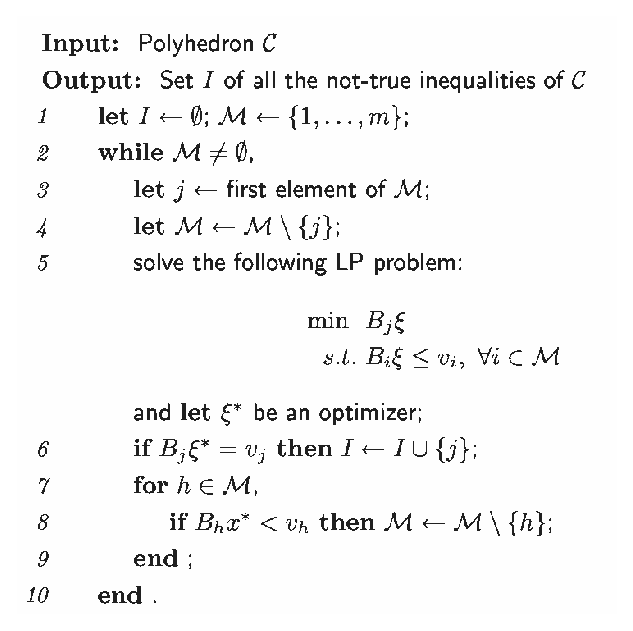
\includegraphics[width=0.6\textwidth]{algorythm1.eps}
     \caption{}
\end{algorithm}

\bigskip
Алгоритм 2 описывает стандартную процедуру для определения размерности $n^{'} \leq n$ наименьшего аффинного подпространства $\mathcal{K}$, содержащего $K^*$, и, когда $n^{'} \leq n$, он находит уравнения, определяющие $\mathcal{K}$. В дальнейшем мы будем предполагать, не теряя общности, что множество $K$ полноразмерно.
\bigskip

\begin{algorithm}[H]
    \SetAlgoLined
    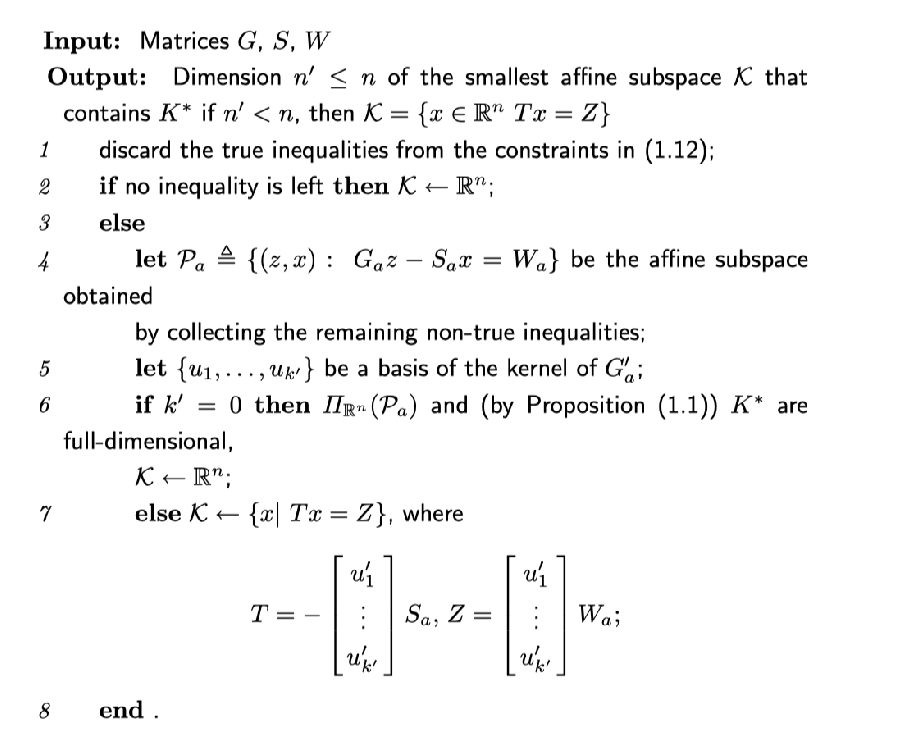
\includegraphics[width=0.8\textwidth]{algorythm2.eps}
     \caption{}
\end{algorithm}


%%%%%%%%%%%%%%%%%%%%%%%%%%%%%%%%%%%%%%%%%%%%%%%%%%%%%%%%%%%%%%%%%%%%%%%%%%%%%%%%
\subsection{Определение критических областей}\label{critical-regions}
%%%%%%%%%%%%%%%%%%%%%%%%%%%%%%%%%%%%%%%%%%%%%%%%%%%%%%%%%%%%%%%%%%%%%%%%%%%%%%%%

В этом разделе мы детализируем алгоритм mp-LP, а именно определение критических областей $CR_{A_i}$ в данном многогранном множестве $K$. Мы предполагаем, что в задачах ЛП нет ни прямой, ни двойственной невырожденности. Обозначим через $z^*: K^* \to \mathbb{R}^s$ функцию оптимизатора, где $Z^* (x) = \{z^* (x)\}$. В этом методе используется прямая выполнимость для получения $H$-полиэдрального представления критических областей, условия ослабления для вычисления оптимизатора $z^* (x)$ и двойственная задача для получения функции оптимального значения $J^* (x)$. Двойственная задача (\ref{1multy}) определяется как

\begin{equation}\label{1critical}
    \begin{split}
       \max_y(W + Sx)^{'}y\\
        \text{при}\ G^{'}y = c,\ y \leq 0.
    \end{split}
\end{equation}
Прямая выполнимость, двойственная выполнимость и условия ослабления для задач (\ref{1multy}), (\ref{1critical}):

\begin{equation}\label{1critical}
    \begin{split}
            PF: Gz \leq W + Sx \\
            DF: G^{'}y = c,\ y \leq 0 \\
            SC: (G_{j}z - W_j - S_{j}x)y_i = 0, \ \forall j \in J \\
            \text{при}\ G^{'}y = c,\ y \leq 0.
        \end{split}
    \end{equation}


Выберем произвольный вектор параметров $x_0 \in \mathcal{K}$ и решим прямую и двойственную задачи (\ref{1multy}), (\ref{1critical}) для $x = x_0$. Пусть $z^*_0$ и $y^*_0$ --- оптимизаторы прямой и двойственной задач соответственно. Значение $z^*_0$ определяет следующее оптимальное разбиение

\begin{equation}\label{2critical}
    \begin{split}
        A(x_0) \triangleq \{ j \in J: G_{j}z^*_0 - S_{j}x_0 - W_j = 0 \}\\
        NA(x_0) \triangleq \{ j \in J: G_{j}z^*_0 - S_{j}x_0 - W_j < 0 \}\\
    \end{split}
\end{equation}
и, следовательно, критическая область $CR_{A (x_0)}$.

По условию $y^*_0$ единственно, а по определению критической области $y^*_0$ остается оптимальным для всех $x \in CR_{A (x_0)}$. Функция значения в $CR_{A (x_0)}$:
\begin{equation}\label{3critical}
   J^*(x) = (W + Sx)^{'}y^*_0
\end{equation}
которая является аффинной функцией $x$ на $CR_{A (x_0)}$, как указано в теореме (\ref{8theorem}). Более того, для оптимального разбиения (\ref{2critical}) условие PF можно переписать в виде:

\begin{equation}\label{4critical}
   G_{A}z^{*}(x) = W_A + S_{A}x
   G_{NA}z^{*}(x) < W_NA + S_{N A}x.
 \end{equation}

В отсутствие двойственной невырожденности прямой оптимизатор является уникальным, и (\ref{4critical}) может быть решена, чтобы получить решение $z^* (x)$. Фактически, уравнения (\ref{4critical}) образуют систему из $l$ равенств, где в отсутствие прямой невырожденности $l = s$ --- число активных ограничений. Из (\ref{4critical}) следует
\begin{equation}\label{4critical}
    z^*(x) = -G^{-1}_{A} S_{A} x + G_{A}^{-1}W_A = Ex + Q,
\end{equation}
откуда следует линейность $z^*$ по $x$. Из условия прямой выполнимости (\ref{4critical}) мы сразу получаем представление критической области $CR_{A (x_0)}$

\begin{equation}\label{4critical}
    G_{NA}(Ex + Q) < W_{NA} + S_{NA}x.
\end{equation}

Как только критическая область $\overline{CR}_{A (x_0)}$ была определена, необходимо исследовать оставшуюся часть пространства $R^{rest} = K \ \backslash \ \overline{CR}_{A (x_0)}$ и создать новые критические области.\\
Эффективный подход к разбиению остального пространства был предложен в \cite{Dua57} и формально доказан в \cite{Bemporad25}. Далее сформулируем теорему, которая оправдывает такую процедуру для характеристики остальной части области $R^{rest}$.

\begin{theorem}\label{9theorem}
    Пусть $Y \subseteq \mathbb{R}^n$ --- многогранник, а $R_0 \triangleq \{x \in Y: Ax \leq b\}$ --- полиэдральное подмножество $Y$, где $b \in R^{m \times 1},\  R_0 \not = \emptyset$. И пусть
    $$R_i = 
    \begin{cases}
        x \in Y: A^{i}x > b^i\\
        A^{j}x \leq b^{j},\ \forall j < i
    \end{cases}
        i = 1,...,m
    $$
    где $b \in \mathbb{R}^{m \times 1}$ и пусть $R^{rest} \triangleq \bigcup^{m}_{i=1} R_i$. Затем

    \begin{equation}\label{1list}
        R^{rest} \cup R_0 = Y
    \end{equation}
    \begin{equation}\label{2list}
        R_0 \cap R_i = \emptyset,\ R_i \cap R_j = \emptyset,\ \forall i \not = j 
    \end{equation}

\end{theorem}

\begin{proof}
    Доказательство: 
    (\ref{1list}). Мы хотим доказать, что если $x \in Y$, то либо $x$ принадлежит $R_0$ или $R_i$ для некоторого $i$. Если $x \in R_0$, мы закончили. В противном случае существует такой индекс $i$, что $A^{i} x > b^i$. Пусть $i^* = \min_{i \leq m} \{ i: A^{i}x > b^{i} \}$. Тогда $x \in R_{i^*}$, $A^{i^{*}} x > b^{i^{*}}$ и $A^{j} x \leq b^{j},\ \forall j < i^*$, по определению $i^*$.
    
    (\ref{2list}). Пусть $x \in R_0.$ Тогда не существует ни одного $i$ такого, что $A^{i} x > b^i$, из чего следует, что $x \in R_i,\  \forall i \leq m$. Пусть $x \in R_i$ и возьмем $i > j$. Поскольку $x \in R_i$, по определению $R_{i} (i > j) A^{j}x \leq b^j$, из чего следует, что $x \not \in R_j$.    
\end{proof}



% %%%%%%%%%%%%%%%%%%%%%%%%%%%%%%%%%%%%%%%%%%%%%%%%%%%%%%%%%%%%%%%%%%%%%%%%%%%%%%%%
% \subsection{Результаты mp-LP алгоритма}
% %%%%%%%%%%%%%%%%%%%%%%%%%%%%%%%%%%%%%%%%%%%%%%%%%%%%%%%%%%%%%%%%%%%%%%%%%%%%%%%%

% Основываясь на приведенном выше обсуждении, решение mp-LP может быть обобщено в следующем алгоритме (\ref{critical-regions}). Обратите внимание, что алгоритм генерирует разбиение пространства состояний в широком смысле. Алгоритм может быть модифицирован для хранения критических областей, как это определено в (\ref{5theorem}), которые являются открытыми наборами, вместо хранения его замыкания. В этом случае алгоритм должен исследовать и хранить все критические области, которые не являются полноразмерными, чтобы создать разделение множества возможных параметров. С практической точки зрения такая процедура не является необходимой, поскольку функция значения и оптимизатор являются непрерывными функциями от $x$.


%%%%%%%%%%%%%%%%%%%%%%%%%%%%%%%%%%%%%%%%%%%%%%%%%%%%%%%%%%%%%%%%%%%%%%%%%%%%%%%%
\section{Multi-Parametric Toolbox}\label{2sec:problem-formulation}
%%%%%%%%%%%%%%%%%%%%%%%%%%%%%%%%%%%%%%%%%%%%%%%%%%%%%%%%%%%%%%%%%%%%%%%%%%%%%%%%

Мы изучаем задачи оптимального управления и построение оптимальной обратной связи. В нашем подходе будет использоваться многопараметрическое программирование, и нашей главной целью будет получение решения с обратной связью по состоянию, а также получение алгоритмов для его эффективного вычисления.

В нашем фреймворке параметрическое программирование является основным методом, используемым для изучения и вычисления законов оптимального управления с обратной связью. Фактически, мы формулируем конечные задачи оптимального управления в виде математических программ, в которых входная последовательность является вектором оптимизации. 
В зависимости от динамической модели системы, характера ограничений и используемой функции, получается другая математическая программа. 
Текущее состояние динамической системы входит в функцию стоимости и ограничения в качестве параметра, который влияет на решение математической программы. 
Мы изучаем структуру решения при изменении этого параметра и описываем алгоритмы решения многопараметрических линейных, квадратичных и смешанных целочисленных программ. 
Они представляют собой основные инструменты для вычисления законов оптимального управления с обратной связью.

Мы показываем, что решение всех этих задач оптимального управления может быть выражено в виде кусочно-афинного закона обратной связи. \\
Кроме того, закон оптимального управления непрерывен, а функция значений выпукла и непрерывна.

Оптимальное управление ограниченными линейно-кусочно-аффинными (PWA) системами получило отличное
интерес к исследовательскому сообществу из-за легкости постановки сложных проблем
и их решения. Целью Multi-Parametric Toolbox (MPT) является предоставление эффективных вычислительных
средства для получения контроллеров обратной связи для типов задач оптимального управления
в среде программирования Matlab. Многопараметрическим программированием, линейным или
задачи квадратичной оптимизации решается в автономном режиме. Соответствующее решение принимает форму
обратной связи штата PWA. В частности, пространство состояний разбивается на многогранные множества и
для каждого из этих наборов закон оптимального управления задается как одна аффинная функция.
Для квадратичных задач, контроллер обратной связи может быть получен для ограниченных
линейных системы с применением методов многопараметрического программирования.
В настоящее время принято аппроксимировать оптимальное управление с ограниченным бесконечным временем (CITOC)
Оптимальное управление кусочно-аффинными системами также вызвало большой интерес к исследованиям.
сообщества, поскольку системы PWA представляют собой мощный инструмент для аппроксимации нелинейных систем и из-за их эквивалентности гибридным системам. Алгоритмы для вычислений
контроллеры с обратной связью для систем PWA с ограничениями были представлены для квадратичного и линейного
цели, а также включены в этот инструментарий.
С помощью контроллеров обратной связи, которые минимизируют конечную стоимость затрат времени, также возможно
получить оптимальное по бесконечному времени решение для систем PWA.
Несмотря на то, что многопараметрические подходы основаны на автономном вычислении закона обратной связи,
вычисление может быстро стать препятствующим для больших проблем. Это связано не только
высокой сложности многопараметрических программ, но в основном из-за
экспоненциального количества переходов между регионами, которые могут произойти, когда контроллер
вычисляется в режиме динамического программирования. 